\subsection{Berechnung der Initialgeschwindigkeit}\label{sec:initialgeschwindigkeit}
Sofern ein Stosskandidat wie in Abschnitt \ref{sec:kandidatensuche} beschrieben gefunden wurde, muss berechnet werden,
welche Geschwindigkeit die weisse Kugel erhalten muss, damit die gewünschte Kugel ins Loch gespielt wird.
Relevant dafür ist der Reibungsverlust, wenn die Kugel rollt und die Kollision mit anderen Kugeln.

Wenn eine Kugel in ein Loch rollen soll, kann eine minimale Endgeschwindigkeit angenommen werden und aufgrund
der zurückzulegenden Strecke die Startgeschwindigkeit bestimmt werden, dies wird in Abschnitt \ref{ReibungsverlustUeberBahn} beschrieben.
Sofern diese Kugel über den Spielball ins Loch gespielt werden soll, muss der Spielball mit einer gewissen
Geschwindigkeit die Kugel treffen, damit diese die gewünschte Startgeschwindigkeit erhält.
Dies wird in Abschnitt \ref{EnergieuebergabeBeiKollision} beschrieben.

\subsubsection{Reibungsverlust über Bahn}\label{ReibungsverlustUeberBahn}
Das Ziel eines Billardstosses ist es, eine Kugel von einem Punkt A zu einem Punkt B rollen zu lassen.
Dabei findet Rollreibung $\mu_r$ sowie Gleitreibung $\mu_g$ statt, welche das Abbremsen der Kugel verursachen.
Die zurückzulegende Strecke sei $\Delta s$ und die Schwerebeschleunigung $g$.
Es ist relevant zu wissen, welche Startgeschwindigkeit $v_1$ eine Kugel am Punkt A haben muss,
um mit der Endgeschwindigkeit $v_2$ am Punkt B anzukommen.
Beispielsweise wenn eine Kugel X in eines der Löcher gespielt werden soll,
wobei die Kugel eine gewisse minimale Endgeschwindigkeit haben soll, damit sie tatsächlich ins Loch rollt.

Es kann die nachfolgende Formel angewendet werden\footnote{Die Herleitung findet sich im Anhang \ref{anhang:herleitung:StartgeschwAnhandEndgeschwMitReibung}}:
\begin{align}
    \vec{v_1} = \sqrt{\frac{49 \cdot \mu_g \cdot (\norm{\vec{v_2}}^2 + 2 \cdot g \cdot \mu_r \cdot \Delta s)}{49 \cdot \mu_g + 24 \cdot (\mu_r - \mu_g)}} \cdot \frac{\vec{v_2}}{\norm{\vec{v_2}}}
\end{align}

Sei $S$ die Startposition der Kugel, $E$ die Endposition der Kugel und $V$ der gewünschte Betrag der Endgeschwindigkeit,
dann lässt sich die Endgeschwindigkeit $\vec{v_2}$ wie folgt berechnen:
\begin{align}
    \vec{\Delta s} = E - S\\
    \hat{\Delta s} = \frac{\vec{\Delta s}}{\norm{\vec{\Delta s}}}\\
    \vec{v_2} = V \cdot \hat{\Delta s}
\end{align}

\subsubsection{Elastischer Stoss bei Kugelkollision}\label{EnergieuebergabeBeiKollision}

Um eine Kugel C in eine gewünschte Richtung, wie etwa zum Loch, rollen zu lassen, muss sie von einer anderen Kugel A,
evtl. vom Spielball, angestossen werden.
Es gilt herauszufinden, wo die Kugel C getroffen werden muss und welche Geschwindigkeit die Kugel A zum Kollisionszeitpunkt
haben muss, um die Kugel C in die gewünschte Richtung mit der geforderten Geschwindigkeit rollen zu lassen.

Die Situation mit der Kugel C an der Position $C$ und der Kugel A, an der Position $A$ ist in Abbildung \ref{fig:ballCollisionPointReverse}
dargestellt.

\begin{figure}[h!]
    \begin{center}
        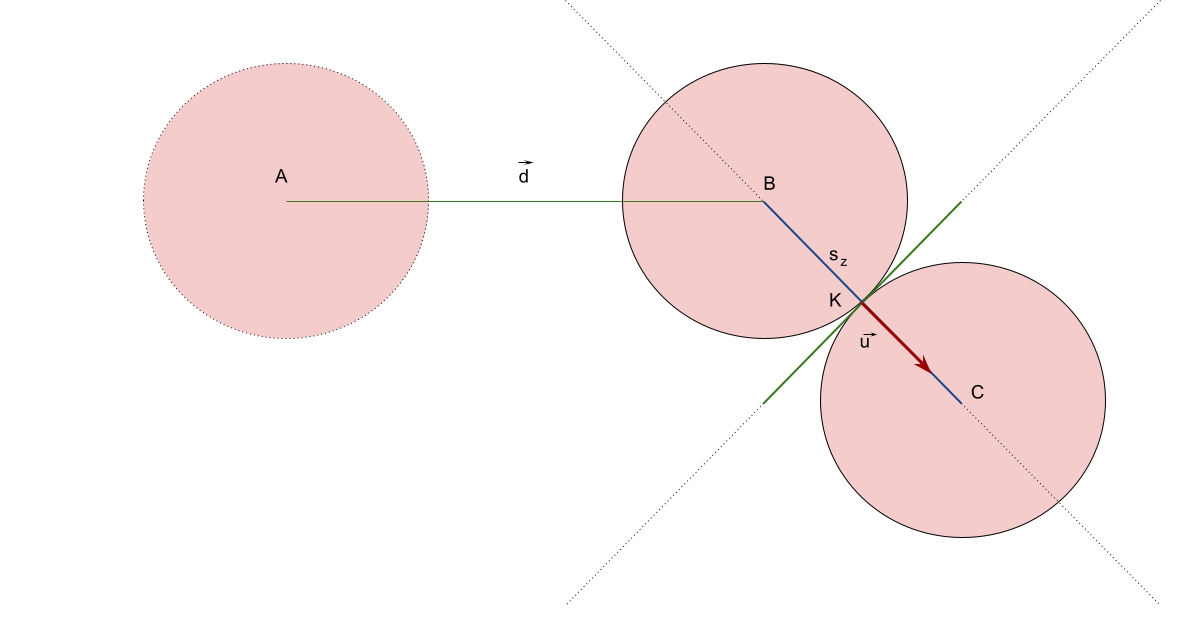
\includegraphics[width=0.6\linewidth]{../common/03_billiard_ai/resources/21_kollisionspunkt_rueckwaerts.png}
    \end{center}
    \caption{Kollisionspunkt zweier Kugeln.
    Die Kugel A muss zum Punkt B rollen, wo sie auf Kugel C prallt und ein elastischer Stoss \cite{wiki.elastischer_stoss_physik:1} stattfindet.
    Während die Kugel die Distanz $\norm{\vec{d}}$ zurücklegt, verliert sie an Geschwindigkeit aufgrund von Reibung,
    diese wird in Abschnitt \ref{ReibungsverlustUeberBahn} behandelt. Hier ist lediglich relevant, welche Geschwindigkeit
    die Kugel A am Punkt $B$ haben muss.
    }
    \label{fig:ballCollisionPointReverse}
\end{figure}

Sei $\vec{u}$, die gewünschte Richtung und Geschwindigkeit der Kugel C nach der Kollision,
dann ist der Zielpunkt $B$ der Kugel A wie folgt definiert\footnote{Die Herleitung findet sich im Anhang \ref{anhang:herleitung:ballCollisionReverse}}:
\begin{align}
    B = C - 2 \cdot r \cdot \hat{u}
\end{align}

Sei $\hat{d}$ der Richtungsvektor der Länge $1$ zwischen den Punkten $A$ und $B$, $E_v$ die Energieverlustkonstante in
Prozent, dann gilt für die Geschwindigkeit $\vec{v_1}$ der Kugel A bei der Kollision\footnote{Die Herleitung findet sich im Anhang \ref{anhang:herleitung:ballCollisionReverse}}:
\begin{align}
    \hat{u} = \frac{\vec{u}}{\norm{\vec{u}}}\\
    \vec{v_1} = \frac{\vec{u} \cdot \vec{u}}{\hat{d} \cdot \vec{u}} \cdot \frac{1}{1 - E_v} \cdot \hat{d}
\end{align}

Anschliessend kann die Startgeschwindigkeit der Kugel A an der Position A berechnet werden, weil die gewünschte
Endgeschwindigkeit und der zurückzulegende Weg bekannt sind\footnote{siehe Kapitel \ref{ReibungsverlustUeberBahn}}.

\subsubsection{Bandenkollision}

Hierbei wird der Geschwindigkeitsvektor berechnet, der vor einer Bandenkollision gilt.
Es wird von einer perfekten Spiegelung ausgegangen. Der an der Bande eingehende
Geschwindigkeitsvektor $\vec{v_0}$ kann demnach berechnet werden, wenn die Bandennormale $\vec{N}$ sowie die
gewünschte Endgeschwindigkeit $\vec{v}$ bekannt ist.
\begin{align}
    \vec{v_0} = \vec{v} - 2 \cdot \vec{N} \cdot (\vec{v} \cdot \vec{N})
\end{align}

Da die Kugel an der Bande Energie verlieren wird,
muss die einkommende Geschwindigkeit $\vec{v_0}$ vor der Bandenkollision um diesen Energieverlust erhöht werden.
\begin{align}
    \vec{v_0} = \norm{\vec{v_0} \cdot \frac{1}{1 - E_v}} \cdot \hat{v_0}
\end{align}